\section{Proofs and Technical Lemmas}
\label{app:theory}

We collect standing identities, shape-constrained facts, and proofs for the results in \Cref{sec:theory}. Unless stated otherwise, expectations are under the logging law $P_{\pi_0}$; $L^2$ norms are with respect to the relevant marginal (e.g., $L^2(P)$ or $L^2(P_S)$). We reuse the fold map $F(\cdot)$ from \Cref{app:folds} and the projection operators from \Cref{app:projections}.

\subsection{Standing identities and tools}
\label{app:theory-tools}

\paragraph{Change of measure.}
For any integrable $h(X,A,S,Y)$ and any candidate $\pi'$,
\begin{equation}
\E\!\big[ W_{\pi'}\, h(X,A,S,Y)\big] \;=\; \E_{\pi'}\!\big[ h(X,A,S,Y)\big],
\qquad \E[W_{\pi'}]=1.
\label{eq:com}
\end{equation}

\paragraph{Doob--Dynkin / conditional expectation as $L^2$ projection.}
Let $\mathcal{G}=\sigma(S)$. Then $m^\star(S):=\E[W_{\pi'}\mid\mathcal{G}]$ is the $L^2$ projection of $W_{\pi'}$ onto the closed subspace $L^2(\mathcal{G})\subset L^2(P)$, i.e.,
\begin{equation}
\E\!\big[(W_{\pi'}-U(S))^2\big]
=\E\!\big[(W_{\pi'}-m^\star(S))^2\big]+\E\!\big[(m^\star(S)-U(S))^2\big],
\label{eq:orth}
\end{equation}
for all $U(S)\in L^2(\mathcal{G})$. In particular, $\Var(W_{\pi'}U)\ge \Var(m^\star(S)U)$ for any $U(S)\in L^2(\mathcal{G})$.

\paragraph{Pythagoras in Hilbert spaces.}
Let $L^2_0(P)$ be the mean-zero Hilbert space with inner product $\langle f,g\rangle=\E[fg]$. For a nonempty closed convex set $\mathcal{C}\subset L^2_0$ and any $z\in L^2_0$, denote by $\Pi_{\mathcal{C}}(z)$ the metric projection. If $\mathcal{C}_1\subseteq \mathcal{C}_2$ then $\mathrm{dist}(z,\mathcal{C}_2)\le \mathrm{dist}(z,\mathcal{C}_1)$.

\subsection{Isotonic regression: mean preservation and majorization}
\label{app:iso-facts}

\begin{lemma}[Mean preservation; PAVA]
\label{lem:iso-mean}
Let $\hat f\in\arg\min_{f\in\mathcal{M}_\uparrow}\sum_{i\in I} (y_i-f(s_i))^2$ be the isotonic fit (PAVA) on indices $I$. Then $\frac{1}{|I|}\sum_{i\in I}\hat f(s_i)=\frac{1}{|I|}\sum_{i\in I}y_i$.
\end{lemma}

\begin{lemma}[Dispersion reduction by majorization]
\label{lem:maj}
After sorting by $s$, the isotonic fitted vector $\hat u$ is a mean-preserving \emph{adjacent pooling} of $y$; hence for any convex $\phi$, $\sum_i \phi(\hat u_i)\le \sum_i \phi(y_i)$ \citep{HardyLittlewoodPolya1952,MarshallOlkinArnold2011}. In particular, with sample mean one, $\Var_n(\hat u)\le \Var_n(y)$ and $\ESS(\hat u)\ge \ESS(y)$.
\end{lemma}

Proofs are standard; see \citet{Ayer1955PAVA,Barlow1972,RobertsonWrightDykstra1988,Banerjee2001}.

\subsection{Proof of \texorpdfstring{\Cref{thm:sur-eif}}{Theorem 1} (surrogate EIF \& variance drop)}
\label{app:proof-sur-eif}
Let $R^\star=\E[Y\mid S]$ and $m^\star(S)=\E[W_{\pi'}\mid S]$. Under mean-sufficiency $\E[Y\mid X,A,S]=R^\star(S)$,
\begin{equation}
V(\pi')=\E\!\big[W_{\pi'}R^\star\big]=\E\!\big[m^\star(S)R^\star(S)\big].
\end{equation}
Standard semiparametric calculations (projecting the unconstrained score onto the tangent space of the surrogate model) yield
\begin{equation}
\phi_{\mathrm{sur}}(O;\pi') = g^\star_{\pi',R}(X)+m^\star(S)\big(R^\star-q^\star_R(X,A)\big)-V(\pi'),
\end{equation}
with $q^\star_R(x,a)=\E[R^\star\mid x,a]$ and $g^\star_{\pi',R}(x)=\E_{A\sim\pi'(\cdot\mid x)}[q^\star_R(x,A)]$ \citep{Bickel1993,VaartWellner2000}. Since $m^\star$ is the $L^2$ projection of $W_{\pi'}$ onto $L^2(\sigma(S))$, Pythagoras (or \eqref{eq:orth}) implies $\Var(\phi_{\mathrm{sur}})\le \Var(\phi_{\mathrm{uncon}})$, strictly unless $W_{\pi'}\in L^2(\sigma(S))$ and $R^\star$ is degenerate.

\subsection{Proof of \texorpdfstring{\Cref{thm:model-restriction}}{Theorem 2} (Efficiency via Model Restriction)}
\label{app:proof-ckp}
Let $\mathcal{M}$ be a baseline semiparametric model with tangent space $T(P)$ and canonical gradient $\phi^\star$.
Let $\mathcal{M}_\mathcal{C} \subset \mathcal{M}$ be a restricted model with tangent space $T_\mathcal{C}(P) \subseteq T(P)$
and canonical gradient $\phi^\star_\mathcal{C}$.

The canonical gradient is defined as the projection of the pathwise derivative onto the tangent space.
Since $T_\mathcal{C}(P) \subseteq T(P)$, we can decompose:
\[
\phi^\star = \phi^\star_\mathcal{C} + \phi^\perp,
\]
where $\phi^\perp \in T(P) \cap T_\mathcal{C}(P)^\perp$ (the orthogonal complement of $T_\mathcal{C}(P)$ within $T(P)$).

By the Pythagorean theorem in Hilbert spaces:
\[
\|\phi^\star\|_2^2 = \|\phi^\star_\mathcal{C}\|_2^2 + \|\phi^\perp\|_2^2 \ge \|\phi^\star_\mathcal{C}\|_2^2,
\]
with equality iff $\phi^\perp = 0$, i.e., $T_\mathcal{C}(P) = T(P)$ (no actual restriction).

Monotonicity for nested restrictions follows: if $T_{\mathcal{C}_1}(P) \supseteq T_{\mathcal{C}_2}(P)$ (i.e., $\mathcal{C}_2$ imposes stronger restrictions, yielding a smaller tangent space), then $\|\phi^\star_{\mathcal{C}_2}\|_2^2 \le \|\phi^\star_{\mathcal{C}_1}\|_2^2$.

For attainability, standard semiparametric arguments apply: one-step corrections or TMLE with cross-fitting
yield regular estimators achieving the restricted efficiency bound \citep{Bickel1993,VaartWellner2000,vanDerLaanRose2011TL}.

\subsection{Proof of \texorpdfstring{\Cref{cor:blackwell}}{Corollary: Blackwell monotonicity}}
\label{app:proof-blackwell}
If $\sigma(S_2)\subseteq\sigma(S_1)$, then $L^2(\sigma(S_2))\subseteq L^2(\sigma(S_1))$.
The surrogate model using $S_1$ has tangent space $T(S_1)$, and the model using $S_2$ has
$T(S_2) \subseteq T(S_1)$ when $\sigma(S_2)\subseteq\sigma(S_1)$.
By \Cref{thm:sur-eif} and the nested-tangent-space argument in \Cref{thm:model-restriction},
the canonical gradient in the smaller tangent space has variance no larger than in the larger one:
$\Var(\phi_{\mathrm{sur}}(S_1))\le \Var(\phi_{\mathrm{sur}}(S_2))$.
Strictness fails only if the finer knowledge already holds, i.e., if $W_{\pi'}$ is $\sigma(S_2)$-measurable and $R^\star$ is degenerate.

\subsection{Proof of \texorpdfstring{\Cref{prop:calips}}{Proposition 1} (Cal-IPS)}
\label{app:proof-calips}
Write
\[
\widehat V_{\IPS}-V(\pi')=(P_n-P)\!\big[m^\star(S)R^\star\big] + P\!\big[(\hat W_{\pi'}-m^\star)R^\star\big]+ P\!\big[m^\star(\hat f(Z(S))-R^\star)\big] + \mathrm{rem},
\]
where $\mathrm{rem}$ collects second-order sample-splitting terms. The empirical process term is $O_p(n^{-1/2})$; the second and third vanish by $L^2$-consistency of weight stabilization and reward calibration (monotone or two-stage) and Cauchy--Schwarz; the remainder is $o_p(1)$ by cross-fitting. Finite-sample dispersion control follows from \Cref{lem:maj} and, if used, the blend cap $\rho\ge1$; under the exact $\mathrm{IsoMeanOne}_S$ projection, $\ESS(\hat W_{\pi'})\ge \ESS(W_{\pi'}^{\mathrm{m1}})$.

\subsection{Proof of \texorpdfstring{\Cref{thm:dr-eff}}{Theorem 3} (Calibrated DR $\sqrt{n}$ limits)}
\label{app:proof-dr}
With cross-fitted nuisances and $R^{\mathrm{OOF}}$ along the IF path,
\[
\widehat V_{\DR}-V(\pi')
= (P_n-P)\!\big[\phi_{\mathrm{sur}}\big]
 + P\!\big[(\hat W_{\pi'}-m^\star)\{q^\star_R-\hat q\}\big]
 + o_p(n^{-1/2}).
\]
The second term is $o_p(n^{-1/2})$ by the one-of-two product-rate condition $\|\hat W_{\pi'}-m^\star\|_2\cdot \|\hat q-q^\star_R\|_2=o_p(n^{-1/2})$ and cross-fitting; the central limit theorem yields the limit variance $\Var(\phi_{\mathrm{sur}})$.

\subsection{Proof of \texorpdfstring{\Cref{thm:budgeted}}{Theorem 4} (budgeted bound)}
\label{app:proof-budget}
Let $\mathcal{W}_\rho=\{m:\E[m]=1,\ m\uparrow S,\ \E[(m-1)^2]\le \rho\,\E[(m^\star-1)^2]\}$. Intersecting the surrogate tangent space with the linear span induced by $m\in\mathcal{W}_\rho$ replaces $m^\star$ by its $L^2(P_S)$ projection $m^\star_\rho=\Pi_{\mathcal{W}_\rho}(m^\star)$ in $\phi_{\mathrm{sur}}$, giving $\phi^{(\rho)}$. Monotonicity in $\rho$ follows from nested convex sets $\mathcal{W}_{\rho_1}\subseteq \mathcal{W}_{\rho_2}$ for $\rho_1\le\rho_2$, and $\lim_{\rho\to\infty}\phi^{(\rho)}=\phi_{\mathrm{sur}}$. If weight stabilization converges to $m^\star_\rho$ (with the same cap), calibrated DR attains $\Var(\phi^{(\rho)})$ by the same one-of-two rate argument.

\subsection{Proof of \texorpdfstring{\Cref{thm:stack}}{Theorem 5} (influence-function stacking) and \texorpdfstring{\Cref{cor:caratheodory}}{Carath\'eodory sparsity}}
\label{app:proof-stack}
Let $\{\widehat V^{(e)}\}$ be regular and asymptotically linear with centered IFs $\{\phi^{(e)}\}$. Set $\Phi=[\phi^{(e)}]$ and $\hat\Sigma=(1/n)\Phi^\top\Phi+\lambda I$. A uniform law of large numbers on the simplex $\Delta$ yields $\hat\Sigma\to\Sigma$ uniformly; by argmin continuity, $\hat\alpha\to\alpha^\star\in\arg\min_{\alpha\in\Delta}\alpha^\top\Sigma\,\alpha$. Hence $\widehat V^{(\hat\alpha)}$ is asymptotically linear with IF $\phi^{(\alpha^\star)}=\sum_e \alpha^\star_e \phi^{(e)}$ and variance $\min_{\alpha\in\Delta}\alpha^\top\Sigma\,\alpha \le \min_e \Sigma_{ee}$. For \Cref{cor:caratheodory}: if $\mathrm{rank}(\Phi)=r$, then the feasible IF combinations lie in an $r$-dimensional affine subspace; by Carath\'eodory's theorem, any point in $\mathrm{conv}\{\phi^{(e)}\}$ admits a representation using at most $r{+}1$ extreme points.

\subsection{Proof of \texorpdfstring{\Cref{prop:oua}}{Proposition 2} (calibration-aware jackknife)}
\label{app:proof-oua}
Let $\widehat V(\hat f)$ be a regular estimator that depends on $f$ only through $R=\hat f(T(S))$, with $f\mapsto \widehat V(f)$ Hadamard-differentiable at $f^\star$ in $L^2(P_S)$. Using a delta-method expansion and cross-fitting (so that oracle folds are asymptotically independent of the IF path), the delete-one-oracle-fold jackknife \citep{Bickel1993,Kunsch1989BlockBootstrap,PolitisRomano1994StationaryBootstrap} consistently estimates the variance contribution from first-stage calibration. Therefore $\widehat{\Var}_{\mathrm{total}}=\widehat{\Var}_{\mathrm{main}}+\widehat{\Var}_{\mathrm{oracle}}$ is consistent for $\Var(\widehat V)$.

\subsection{Auxiliary lemmas used in the main proofs}
\label{app:aux}

\begin{lemma}[OOF mean preservation for reward calibration]
\label{lem:oof-mean}
Let $K$ be fixed and let $R^{\mathrm{OOF}}_i=\hat f^{(-F(i))}(Z(S_i))$ be OOF predictions from reward calibration (either mode). Then $P_n[R^{\mathrm{OOF}}]-P_n[Y]=o_p(1)$ and $P[R^{\mathrm{OOF}}-R^\star]=o_p(1)$ under $L^2(P_S)$-consistency of $\hat f$.
\end{lemma}

\begin{lemma}[Second-order remainder for DR with cross-fitting]
\label{lem:remainder}
Let $\widehat V_{\DR}$ be calibrated DR with cross-fitted $(\hat q,\hat g_{\pi'})$ and calibrated $\hat W_{\pi'}$. Then
\[
\widehat V_{\DR}-V(\pi')-(P_n-P)\phi_{\mathrm{sur}}
= P\!\big[(\hat W_{\pi'}-m^\star)(q^\star_R-\hat q)\big]+o_p(n^{-1/2}),
\]
and the bracketed term is $o_p(n^{-1/2})$ under $\|\hat W_{\pi'}-m^\star\|_2\cdot \|\hat q-q^\star_R\|_2=o_p(n^{-1/2})$.
\end{lemma}

\begin{lemma}[Guard stability]
\label{lem:guard}
Let $W^{\mathrm{stack}}$ be the OOF-stacked candidate and $W^{\mathrm{m1}}_{\pi'}$ the mean-one baseline. For $\rho\ge1$, define $\alpha=\min\!\big\{1,\sqrt{\rho\,\Var(W^{\mathrm{m1}}_{\pi'})/\Var(W^{\mathrm{stack}})}\big\}$ and $W^{\mathrm{blend}}=1+\alpha(W^{\mathrm{stack}}-1)$. Then $\Var(W^{\mathrm{blend}})=\alpha^2\Var(W^{\mathrm{stack}})\le \rho\,\Var(W^{\mathrm{m1}}_{\pi'})$, and the subsequent mean-one isotonic projection cannot increase empirical variance by \Cref{lem:maj}.
\end{lemma}

\emph{Implementation note.} The reference implementation uses a simpler absolute-cap formula $\alpha=\min\{1,\sqrt{\rho/\Var(W^{\mathrm{stack}})}\}$ and omits the final isotonic re-projection (normalizing to mean one instead). This relaxation empirically yields similar ESS improvements but does not carry the deterministic guarantee of \Cref{lem:guard}.

\begin{lemma}[Firm non-expansiveness of projections]
\label{lem:firm}
Metric projections onto closed convex sets in Hilbert spaces are firmly non-expansive:
$\|\Pi_{\mathcal{C}}(x)-\Pi_{\mathcal{C}}(y)\|^2 \le \langle \Pi_{\mathcal{C}}(x)-\Pi_{\mathcal{C}}(y),\, x-y\rangle$.
Hence compositions of projection modules (reward, weight, IF-space projections) are non-expansive. See, e.g., \citet[Prop.~4.16]{BauschkeCombettes2017}.
\end{lemma}

\paragraph{Remarks on dependence.}
If logs exhibit serial or cluster dependence, the IF CLTs can be replaced by block/stationary bootstrap arguments; our reported intervals can include a dependence-robust alternative (App.~\ref{app:diagnostics-defs}).

\subsection{Coverage-Limited Efficiency (CLE) bound}
\label{app:proof-cle}

We derive the CLE bound stated in \cref{eq:cle-bound}. Let $\mathcal{T} \subset \mathcal{X} \times \mathcal{A}$ be a target-relevant region with $\alpha = P_{\pi'}(\mathcal{T})$ and $\beta = P_{\pi_0}(\mathcal{T})$.

\begin{lemma}[Weight second moment on $\mathcal{T}$]
\label{lem:weight-identity}
For the normalized conditional distributions $\pi'_{\mathcal{T}}$ and $\pi_{0,\mathcal{T}}$,
\[
\E_{\pi_0}\!\big[W_{\pi'}^2\, \ind{\mathcal{T}}\big] = \frac{\alpha^2}{\beta}\bigl(1 + \chi^2(\pi'_{\mathcal{T}} \| \pi_{0,\mathcal{T}})\bigr).
\]
\end{lemma}
\begin{proof}
By definition of $\chi^2$ divergence for the normalized conditionals:
$\chi^2(\pi'_{\mathcal{T}} \| \pi_{0,\mathcal{T}}) = \int_{\mathcal{T}} \frac{(d\pi'_{\mathcal{T}})^2}{d\pi_{0,\mathcal{T}}} - 1
= \frac{\beta}{\alpha^2} \int_{\mathcal{T}} \frac{(d\pi')^2}{d\pi_0} - 1
= \frac{\beta}{\alpha^2} \E_{\pi_0}[W_{\pi'}^2 \ind{\mathcal{T}}] - 1$.
Rearranging gives the stated identity.
\end{proof}

\begin{proposition}[CLE bound for IPS-style estimators]
\label{prop:cle}
For any IPS-style estimator $\hat\Psi_{\mathrm{IPS}}$ of $V(\pi') = \E_{\pi'}[Y]$ based on importance-weighted outcomes,
\[
\SE(\hat\Psi_{\mathrm{IPS}}) \;\ge\; \frac{\sigma_{\mathcal{T}}\, \alpha}{\sqrt{\beta\, n}}\, \sqrt{1 + \chi^2(\pi'_{\mathcal{T}} \| \pi_{0,\mathcal{T}})},
\]
where $\sigma_{\mathcal{T}}^2 := \mathrm{ess\,inf}_{(x,a)\in \mathcal{T}} \Var(Y \mid X{=}x, A{=}a)$ is the minimal outcome noise in $\mathcal{T}$.
\end{proposition}

\begin{proof}
We lower bound $\Var_{\pi_0}(W_{\pi'} Y)$ using the Law of Total Variance, conditioning on $(X,A)$:
\[
\Var_{\pi_0}(W_{\pi'} Y) = \E_{\pi_0}[\Var(W_{\pi'} Y \mid X,A)] + \Var_{\pi_0}(\E[W_{\pi'} Y \mid X,A]).
\]
Since $W_{\pi'}$ is $(X,A)$-measurable:
\begin{align*}
\Var(W_{\pi'} Y \mid X,A) &= W_{\pi'}^2 \Var(Y \mid X,A), \\
\E[W_{\pi'} Y \mid X,A] &= W_{\pi'} \E[Y \mid X,A].
\end{align*}
Dropping the non-negative second term:
\[
\Var_{\pi_0}(W_{\pi'} Y) \ge \E_{\pi_0}[W_{\pi'}^2 \Var(Y \mid X,A)].
\]
Restricting to $\mathcal{T}$ (non-negative integrand) and applying $\Var(Y \mid X,A) \ge \sigma_{\mathcal{T}}^2$ on $\mathcal{T}$:
\[
\E_{\pi_0}[W_{\pi'}^2 \Var(Y \mid X,A)] \ge \sigma_{\mathcal{T}}^2 \E_{\pi_0}[W_{\pi'}^2 \ind{\mathcal{T}}].
\]
Applying \Cref{lem:weight-identity}:
\[
\Var_{\pi_0}(W_{\pi'} Y) \ge \frac{\sigma_{\mathcal{T}}^2 \alpha^2}{\beta}(1 + \chi^2).
\]
The asymptotic variance of IPS is $\Var_{\pi_0}(W_{\pi'} Y)/n$; taking square roots yields the stated bound.
\end{proof}

\paragraph{Interpretation.}
The CLE bound has three multiplicative factors:
(i) the \textbf{coverage penalty} $\alpha/\sqrt{\beta}$, which explodes when the logger rarely visits target-typical regions ($\beta \ll \alpha$);
(ii) the \textbf{shape mismatch} $\sqrt{1+\chi^2}$, which inflates the floor even with good coverage if the target concentrates differently within $\mathcal{T}$;
(iii) the standard \textbf{noise term} $\sigma_{\mathcal{T}}/\sqrt{n}$.

\paragraph{Corollary (ESS form).}
Using $\ESS(W_{\pi'}) = n / (1 + \CV^2(W_{\pi'}))$ and the relationship between $\chi^2$ and ESS on $\mathcal{T}$:
\[
\SE(\hat\Psi) \;\ge\; \frac{\sigma_{\mathcal{T}}}{\sqrt{\ESS_{\mathcal{T}}}},
\]
where $\ESS_{\mathcal{T}}$ is the effective sample size \emph{restricted to} $\mathcal{T}$. This shows that high global ESS is insufficient: what matters is ESS in target-relevant regions.

\subsection{TTC collapse with sequence length (structural coverage sparsity)}
\label{app:ttc-collapse}

Even with \emph{perfect} propensity estimates (no teacher-forcing noise), logger coverage collapses exponentially with sequence length. This formalizes why logs-only OPE is fundamentally impractical for open-ended generation, independent of TF brittleness.

\begin{proposition}[Exponential collapse of logger coverage]
\label{prop:ttc-collapse}
Let $q$ and $p$ be token-level distributions with $\mathrm{KL}(p \| q) = \delta > 0$ per token.
For i.i.d.\ sequences of length $L$, the trajectory-level KL divergence is $L \delta$, and
\[
\mathrm{TTC} := P_{\pi_0}(\text{target-typical region}) \;\le\; \exp\bigl(-\Omega(L \delta)\bigr).
\]
When $L \delta \gg 1$, logger coverage is exponentially small in $L$.
\end{proposition}

\begin{proof}[Sketch]
Under the product measure, trajectory log-likelihood ratios concentrate around $L \cdot \E_p[\log(p/q)] = L \delta$.
By standard large-deviation arguments (Sanov's theorem), the probability that a logger-sampled trajectory falls in the target-typical region decays as $\exp(-L \cdot D)$ for some $D > 0$ depending on $\delta$.
\end{proof}

\paragraph{Simulation verification.}
\Cref{fig:ttc-collapse} demonstrates this collapse empirically. We simulate sequences of length $L \in \{25, 50, 100, 200, 400\}$ with Zipf-distributed tokens ($V{=}1000$, $\alpha{=}1.2$) and reward-tilted target policies ($\eta \in \{0.1, 0.3, 0.5\}$, corresponding to small/medium/large shifts). Outcomes $Y = u_{a_0} + \varepsilon$ depend on the first token's utility (modeling a judge score with constant variance regardless of response length). Even with \emph{exact} importance weights (no TF noise), TTC collapses from $>0.8$ at $L=25$ to $<0.01$ at $L=400$ for $\eta \geq 0.3$. For medium and large shifts, IPS RMSE grows 20--50$\times$ with sequence length (from ${\sim}0.02$ to ${\sim}0.5$); for small shifts where TTC remains above 0.70, IPS stays closer to Direct. Direct RMSE remains flat at ${\sim}0.01$ regardless of sequence length or policy shift.

\begin{figure}[t]
  \centering
  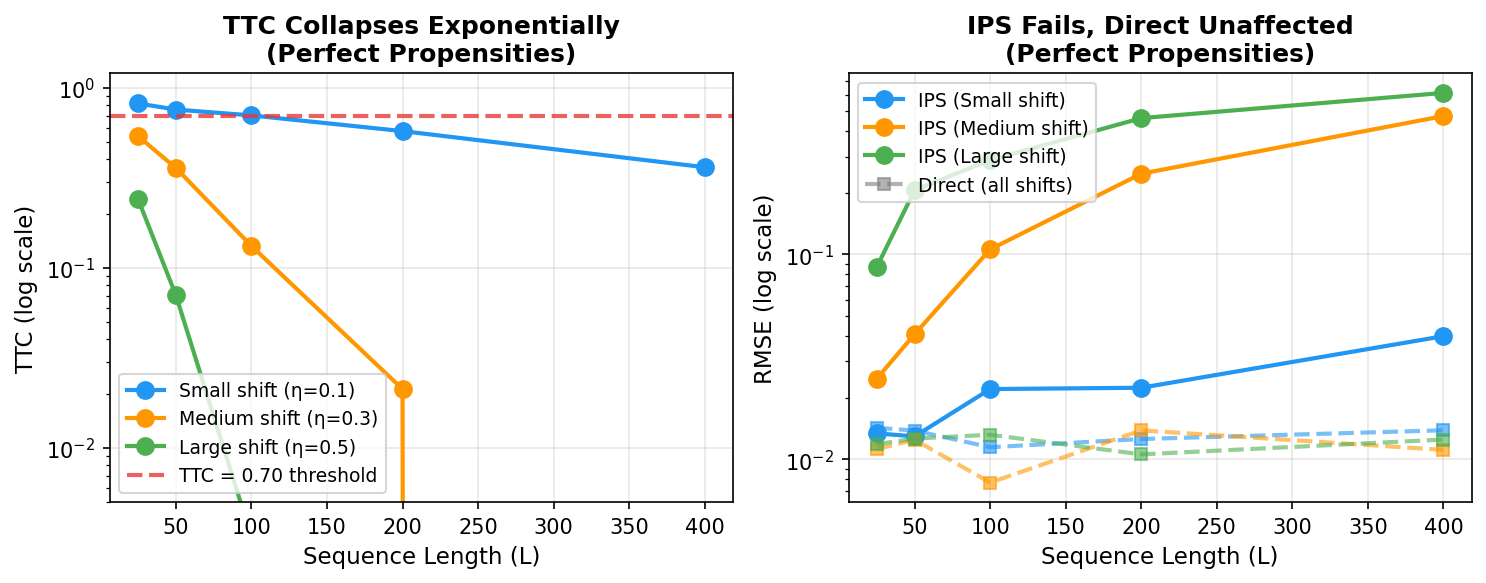
\includegraphics[width=\columnwidth]{figs/ttc_collapse_simulation.png}
  \caption{\textbf{TTC collapse with sequence length---even with perfect propensities.} Left: TTC decreases exponentially with $L$ for all policy shifts $\eta > 0$; only the smallest shift ($\eta{=}0.1$) stays above the 0.70 threshold beyond $L{=}100$. Right: For medium/large shifts, IPS RMSE (solid) grows 20--50$\times$ with $L$; for small shifts where TTC ${\geq} 0.70$, IPS stays closer to Direct. Direct RMSE (dashed) remains flat at ${\sim}0.01$ regardless of $L$. This demonstrates that coverage sparsity is a \emph{structural} limitation of autoregressive trajectory spaces, not a bug in propensity estimation.}
  \label{fig:ttc-collapse}
\end{figure}

\emph{Implication.} For open-ended LLM generation with typical response lengths ($L \approx 100$--$500$ tokens), even tiny per-token KL divergence ($\delta \approx 0.03$ nats) yields negligible TTC. This is not a TF bug---it is the geometry of high-dimensional trajectory spaces. Logs-only OPE faces a \emph{structural} precision floor that no estimator can overcome.

\subsection{EIF derivation for Direct mode}
\label{app:eif-direct}

Direct mode estimates $\theta := \E[Y]$ when oracle labels are observed only for a subset $L \subset [n]$.
Let $L_i \in \{0,1\}$ indicate oracle observation, and assume missing at random (MAR):
$\Pr(L_i=1 \mid Z_i, Y_i) = \Pr(L_i=1 \mid Z_i) =: e(Z_i)$, where $Z_i$ is the calibration index.
Under this model, the efficient influence function for $\theta$ is \citep{Tsiatis2006,BangRobins2005}:
\[
  \phi(O_i) = \mu(Z_i) - \theta + \frac{L_i}{e(Z_i)}\bigl(Y_i - \mu(Z_i)\bigr),
\]
where $\mu(z) := \E[Y \mid Z=z]$.
Averaging this EIF with estimated $(\hat\mu, \hat e)$ yields the one-step estimator.
In our setting, oracle inclusion is approximately uniform, so $\hat e(Z_i) \approx |L|/n$, giving:
\[
  \hat\theta_{\mathrm{aug}} = \frac{1}{n}\sum_{i=1}^n \hat\mu(Z_i) + \frac{1}{|L|}\sum_{i \in L}\bigl(Y_i - \hat\mu^{(-i)}(Z_i)\bigr),
\]
which matches \cref{eq:theta-aug}. The cross-fit predictions $\hat\mu^{(-i)}$ avoid overfitting bias in the residual term.

\emph{Remark (TMLE equivalence).} The cross-fitted augmented estimator $\hat\theta_{\mathrm{aug}}$ is the one-step/AIPW estimator for the EIF above, specializing to $e(Z) \approx |L|/n$ under approximately uniform oracle sampling. A TMLE that targets $\hat\mu$ via a logistic fluctuation using clever covariate $H(O) = L/e(Z)$ (equivalently, $H(Z) = 1/e(Z)$ on labeled rows) solves the EIF estimating equation and is asymptotically equivalent to $\hat\theta_{\mathrm{aug}}$, yielding the same influence function and achieving the semiparametric efficiency bound for $\theta$ in the MAR model \citep{vanDerLaanRose2011TL}.

\subsection{Assumptions and what CJE relaxes}
\label{app:assumptions-ledger}

CJE's key innovation is replacing untestable identification assumptions with auditable diagnostics. We organize assumptions into four categories, with \textbf{mean transport} as the fundamental identification requirement.

\paragraph{A0 (Bridge Assumption).}
$\E[Y^* \mid X, A] = \E[Y \mid X, A]$. The operational oracle $Y$ is sufficiently aligned with the idealized deliberation oracle $Y^*$ such that optimizing for $Y$ approximates optimizing for $Y^*$. This is a governance question outside the statistical framework---oracle selection requires domain expertise and construct validity audits.

\paragraph{Category A: Design/missingness requirements (always needed).}
\begin{itemize}[leftmargin=*,nosep]
\item \textbf{Oracle MAR (L1):} $L \perp Y \mid (X, A, S)$. Oracle labeling is ignorable conditional on observed data.
\item \textbf{Oracle positivity (L2):} $P(L=1 \mid X, A, S) > 0$ on the support where calibration will be applied.
\end{itemize}

\paragraph{Category B: Identification for surrogate-only mean claims (the fundamental requirement).}
The requirement for valid policy value estimation is \textbf{mean transport}:
\[
\E_{\pi'}[Y - f(S,X)] = 0.
\]
This is exactly the condition tested by the mean residual audit (\cref{prop:mean-transport}). CJE treats transport as testable rather than assumed:
\begin{itemize}[leftmargin=*,nosep]
\item \textbf{With audit} (${\sim}50$--$200$ oracle labels per $\pi'$): Test transport directly. Pass $\to$ reuse calibration; fail $\to$ recalibrate or refuse level claims.
\item \textbf{Without audit}: Transport must be assumed. In our experiments, calibration transported well across comparable policies (clone, premium, prompt-engineered) but failed for adversarial ones. How aggressively you audit depends on context---stakes, policy similarity, and historical transport stability.
\end{itemize}

\paragraph{Category C: Structural assumptions (sufficient for transport, not required).}
The following are \emph{sufficient conditions} that imply transport. CJE does not require them when transport is verified via audit:
\begin{itemize}[leftmargin=*,nosep]
\item \textbf{Prentice-style surrogacy:} $Y \perp A \mid (X, S)$ (distributional stability across policies).
\item \textbf{Mean sufficiency / single-index (J2-M, J2-SI):} $\E[Y \mid X, A, S] = \mu(g(S,X))$ for some monotone $\mu$ and index $g$.
\end{itemize}
These structural assumptions also enable the efficiency theory (\cref{thm:sur-eif,thm:dr-eff}), but are not required for consistent estimation when transport is audited. Mean sufficiency implies transport (if it holds globally), but transport can hold without it---errors may cancel in expectation even when the structural assumption fails.

\paragraph{Category D: Estimator-dependent requirements.}
\textbf{Overlap (S3):} $\pi'(a \mid x) > 0 \Rightarrow \pi_0(a \mid x) > 0$. Required for IPS and DR estimators. The Direct method requires no overlap---it generates fresh responses under $\pi'$.

\emph{Diagnostic:} Target-Typicality Coverage (TTC). If TTC $< 0.7$, logs-only IPS will fail due to coverage-limited efficiency; prefer Direct.

\subsection{Additional corollaries}
\label{app:additional-corollaries}

\begin{corollary}[Blackwell-efficiency monotonicity]
\label{cor:blackwell}
If $S_2$ is a garbling of $S_1$ (i.e., $\sigma(S_2)\subseteq\sigma(S_1)$), then
$\Var\!\big(\phi_{\mathrm{sur}}(S_1)\big)\le \Var\!\big(\phi_{\mathrm{sur}}(S_2)\big)$,
with strict inequality unless $W_{\pi'}$ is already $\sigma(S_2)$-measurable and $R^\star$ is degenerate.
This is a statistical analog of Blackwell's theorem on experiment comparisons \citep{Blackwell1953}: finer information structures dominate coarser ones.
\end{corollary}

\begin{corollary}[Carath\'eodory sparsity]
\label{cor:caratheodory}
If $\Phi=[\phi^{(e)}]$ has empirical rank $r$, the variance-optimal convex combination uses at most $r{+}1$
base estimators.
\end{corollary}

\subsection{What the bounds do not include}
\label{app:not-in-bounds}
The surrogate and budgeted information bounds describe \emph{model} limits: they do not include (i) finite-sample dispersion control from the sample cap (we encode it population-wise via $\rho$) or (ii) the oracle first-stage uncertainty (added separately by calibration-aware inference).

\subsection{Budgeted bound and IF stacking (OPE-specific results)}
\label{app:budgeted-stacking}

The following results apply to off-policy evaluation (IPS and DR estimators). Direct mode does not use importance weights and is unaffected by these bounds.

\paragraph{Budgeted bound (variance cap).}
For $\rho\ge 1$, define
\[
\mathcal{W}_\rho \;=\; \Big\{ m:\ \E[m]=1,\; m\uparrow S,\; \E\big[(m-1)^2\big]\le
\rho\,\E\big[(m^\star-1)^2\big]\Big\},
\]
and let $m^\star_\rho$ be the $L^2(P_S)$ projection of $m^\star$ onto $\mathcal{W}_\rho$.
Define the budgeted gradient
$\phi^{(\rho)}= g^\star_{\pi',R}(X) + m^\star_\rho(S)\big(R^\star-q^\star_R(X,A)\big) - V(\pi')$.

\begin{theorem}[Budgeted information bound]
\label{thm:budgeted}
The optimal asymptotic variance under the cap $\rho$ equals $\Var(\phi^{(\rho)})$,
which is nonincreasing in $\rho$ and satisfies
$\lim_{\rho\to\infty}\Var(\phi^{(\rho)})=\Var(\phi_{\mathrm{sur}})$.
If weight stabilization converges to $m^\star_\rho$ (with the guard), then calibrated DR attains $\Var(\phi^{(\rho)})$.
\end{theorem}

\noindent\emph{In plain terms:} This formalizes ``don't let weights explode.'' Limiting weight variance ($\rho$) trades a bit of asymptotic efficiency for much better finite-sample behavior.

\begin{theorem}[Influence-function stacking]
\label{thm:stack}
Let $\{\widehat V^{(e)}\}_{e\in\mathcal{E}}$ be regular, asymptotically linear estimators with centered IFs
$\{\phi^{(e)}\}$, and let $\hat\alpha\in\arg\min_{\alpha\in\Delta}\alpha^\top \hat\Sigma\,\alpha$ with
$\hat\Sigma$ the empirical IF covariance. If $\hat\Sigma\to \Sigma$ uniformly on $\Delta$, then the
stacked estimator $\widehat V^{(\hat\alpha)}$ is asymptotically linear with IF $\phi^{(\alpha^\star)}$ and
variance $\min_{\alpha\in\Delta}\alpha^\top \Sigma\,\alpha\le \min_e \Sigma_{ee}$.
An outer split leaves the limit unchanged. (This extends ensemble learning from prediction, where Super Learner \citep{vanderLaan2007SuperLearner} combines algorithms to minimize cross-validated risk, to asymptotic efficiency: we combine estimators by minimizing the variance of their combined influence function.)
\end{theorem}

